%!TEX root = report.tex	
\begin{subfigure}{0.16\textwidth}
	\centering
	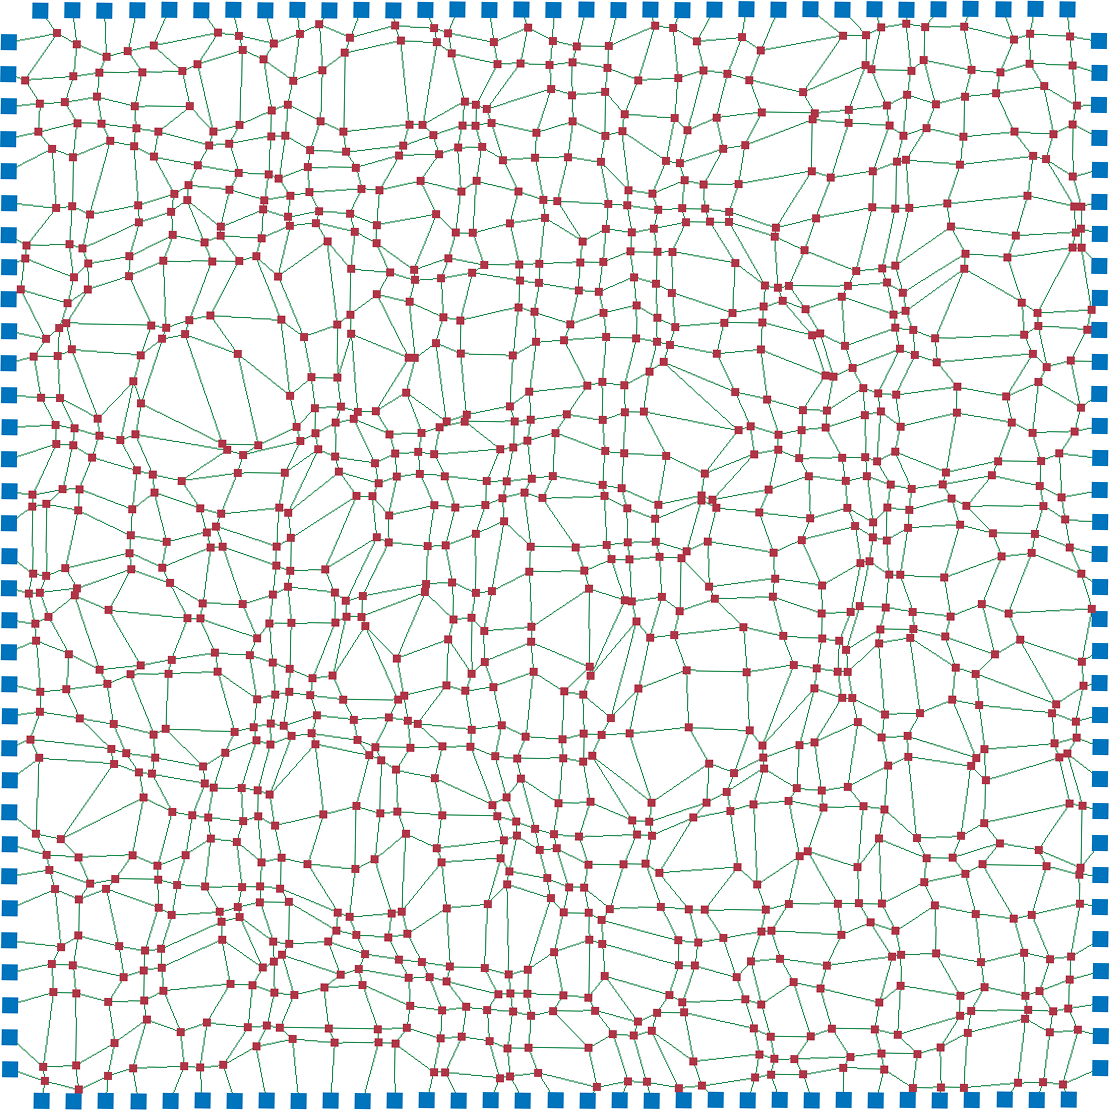
\includegraphics[
		width=\textwidth, 
		height=\textwidth, 
		keepaspectratio=true]
	{./img/results/1200_0_1_stretchHighest_97_step_0}
	%\caption{Step 0}
	%\label{fig:experiment:stretchHighestStrain:0}
\end{subfigure}	
\begin{subfigure}{0.16\textwidth}
	\centering
	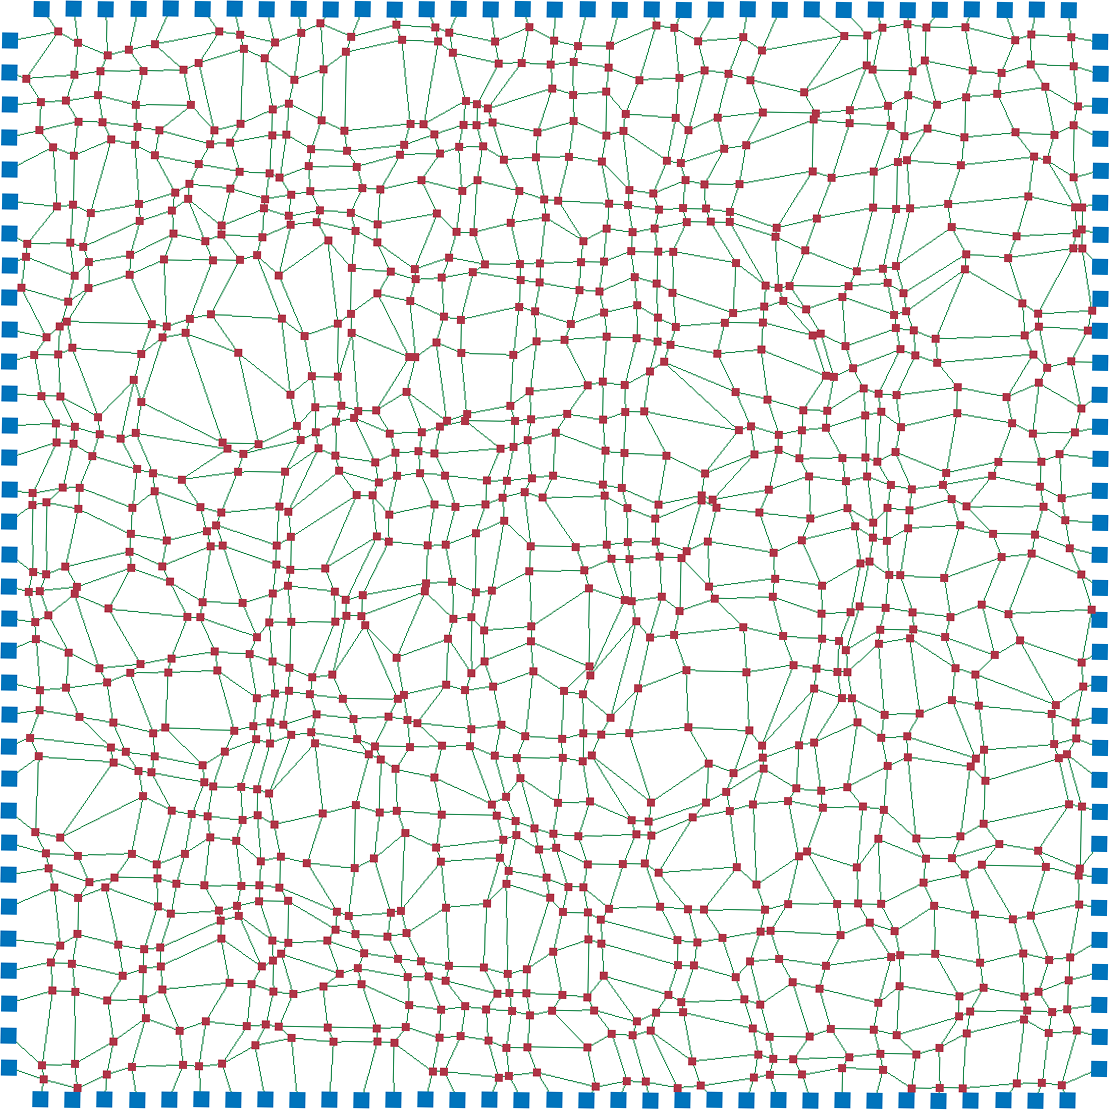
\includegraphics[
		width=\textwidth, 
		height=\textwidth, 
		keepaspectratio=true]
	{./img/results/1200_0_1_stretchHighest_97_step_1}
	%\caption{Step 1}
	%\label{fig:experiment:stretchHighestStrain:1}
\end{subfigure}		
\begin{subfigure}{0.16\textwidth}
	\centering
	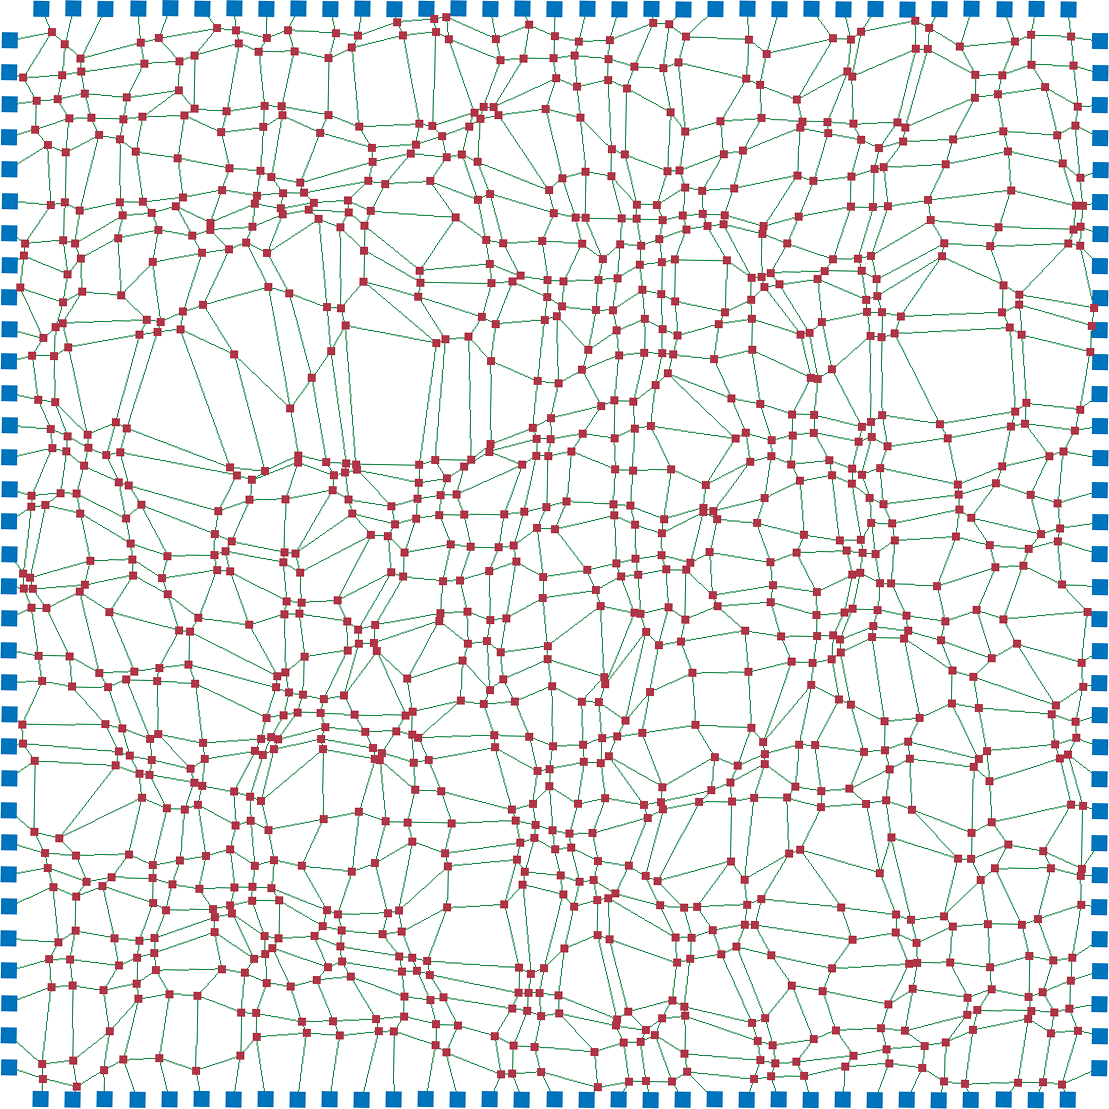
\includegraphics[
		width=\textwidth, 
		height=\textwidth, 
		keepaspectratio=true]
	{./img/results/1200_0_1_stretchHighest_97_step_2}
	%\caption{Step 2}
	%\label{fig:experiment:stretchHighestStrain:2}
\end{subfigure}			
\begin{subfigure}{0.16\textwidth}
	\centering
	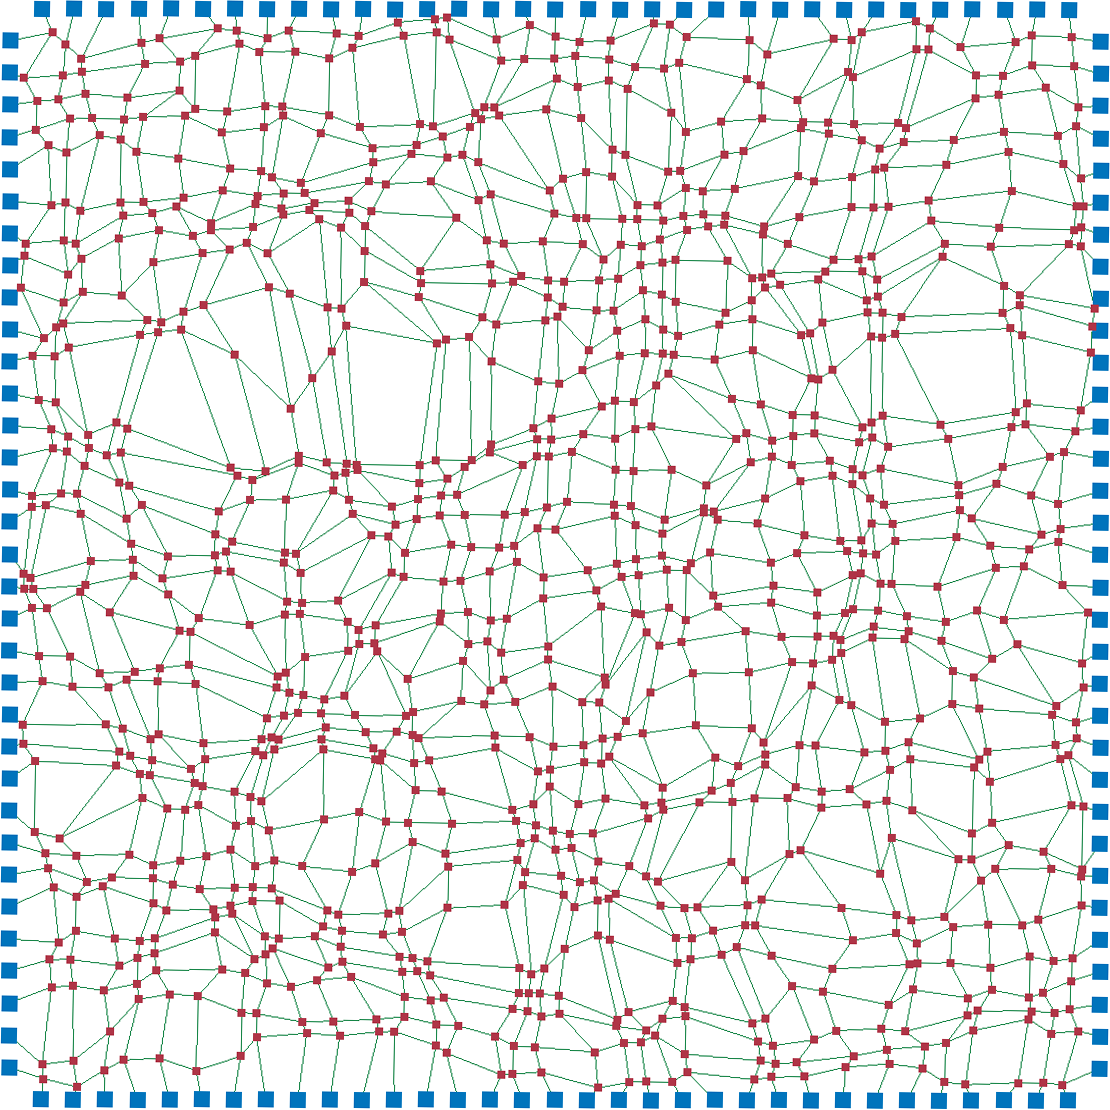
\includegraphics[
		width=\textwidth, 
		height=\textwidth, 
		keepaspectratio=true]
	{./img/results/1200_0_1_stretchHighest_97_step_3}
	%\caption{Step 3}
	%\label{fig:experiment:stretchHighestStrain:3}
\end{subfigure}				
\begin{subfigure}{0.16\textwidth}
	\centering
	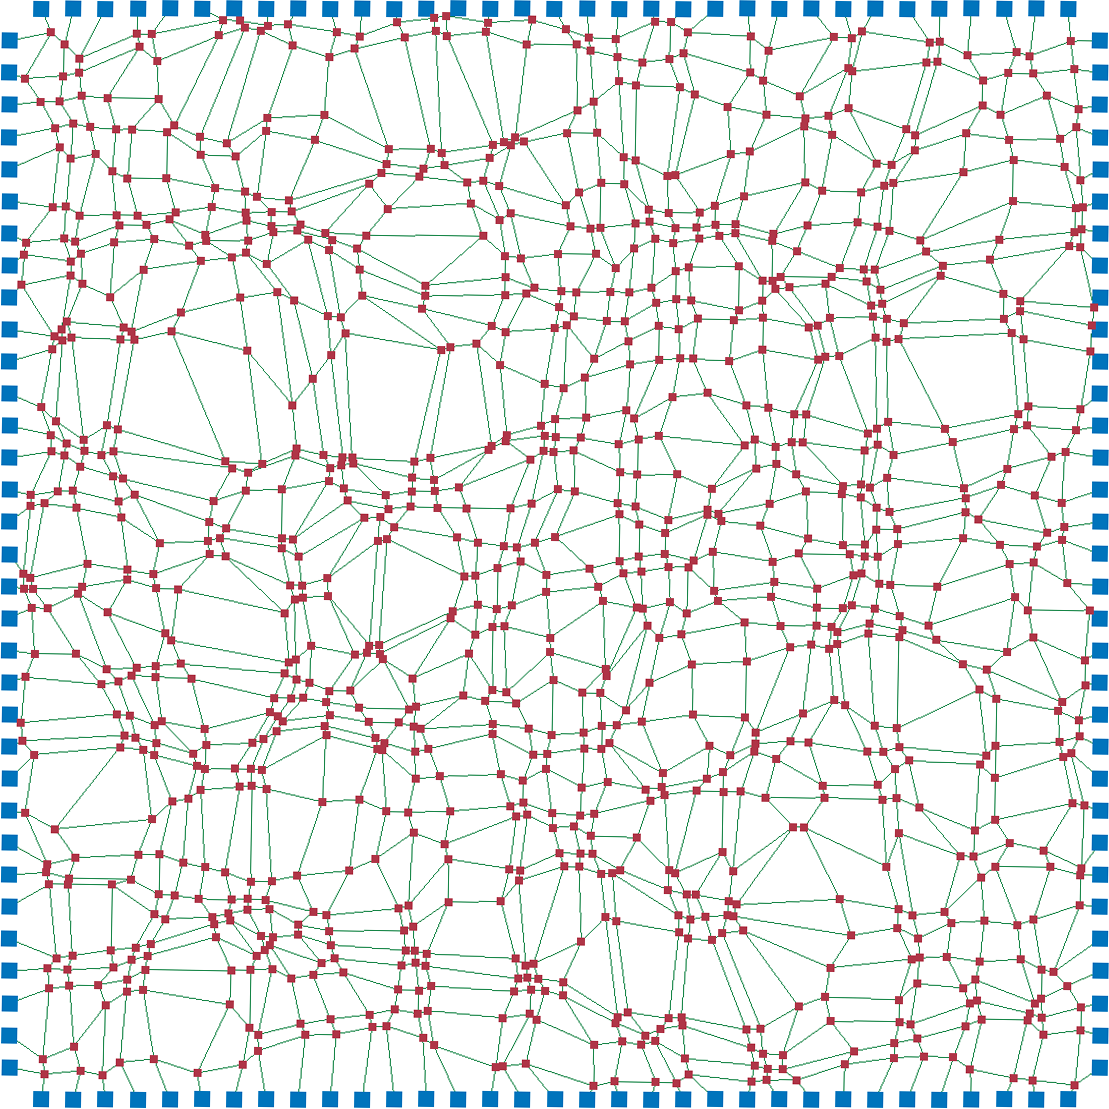
\includegraphics[
		width=\textwidth, 
		height=\textwidth, 
		keepaspectratio=true]
	{./img/results/1200_0_1_stretchHighest_97_step_4}
	%\caption{Step 4}
	%\label{fig:experiment:stretchHighestStrain:4}
\end{subfigure}
\begin{subfigure}{0.16\textwidth}
	\centering
	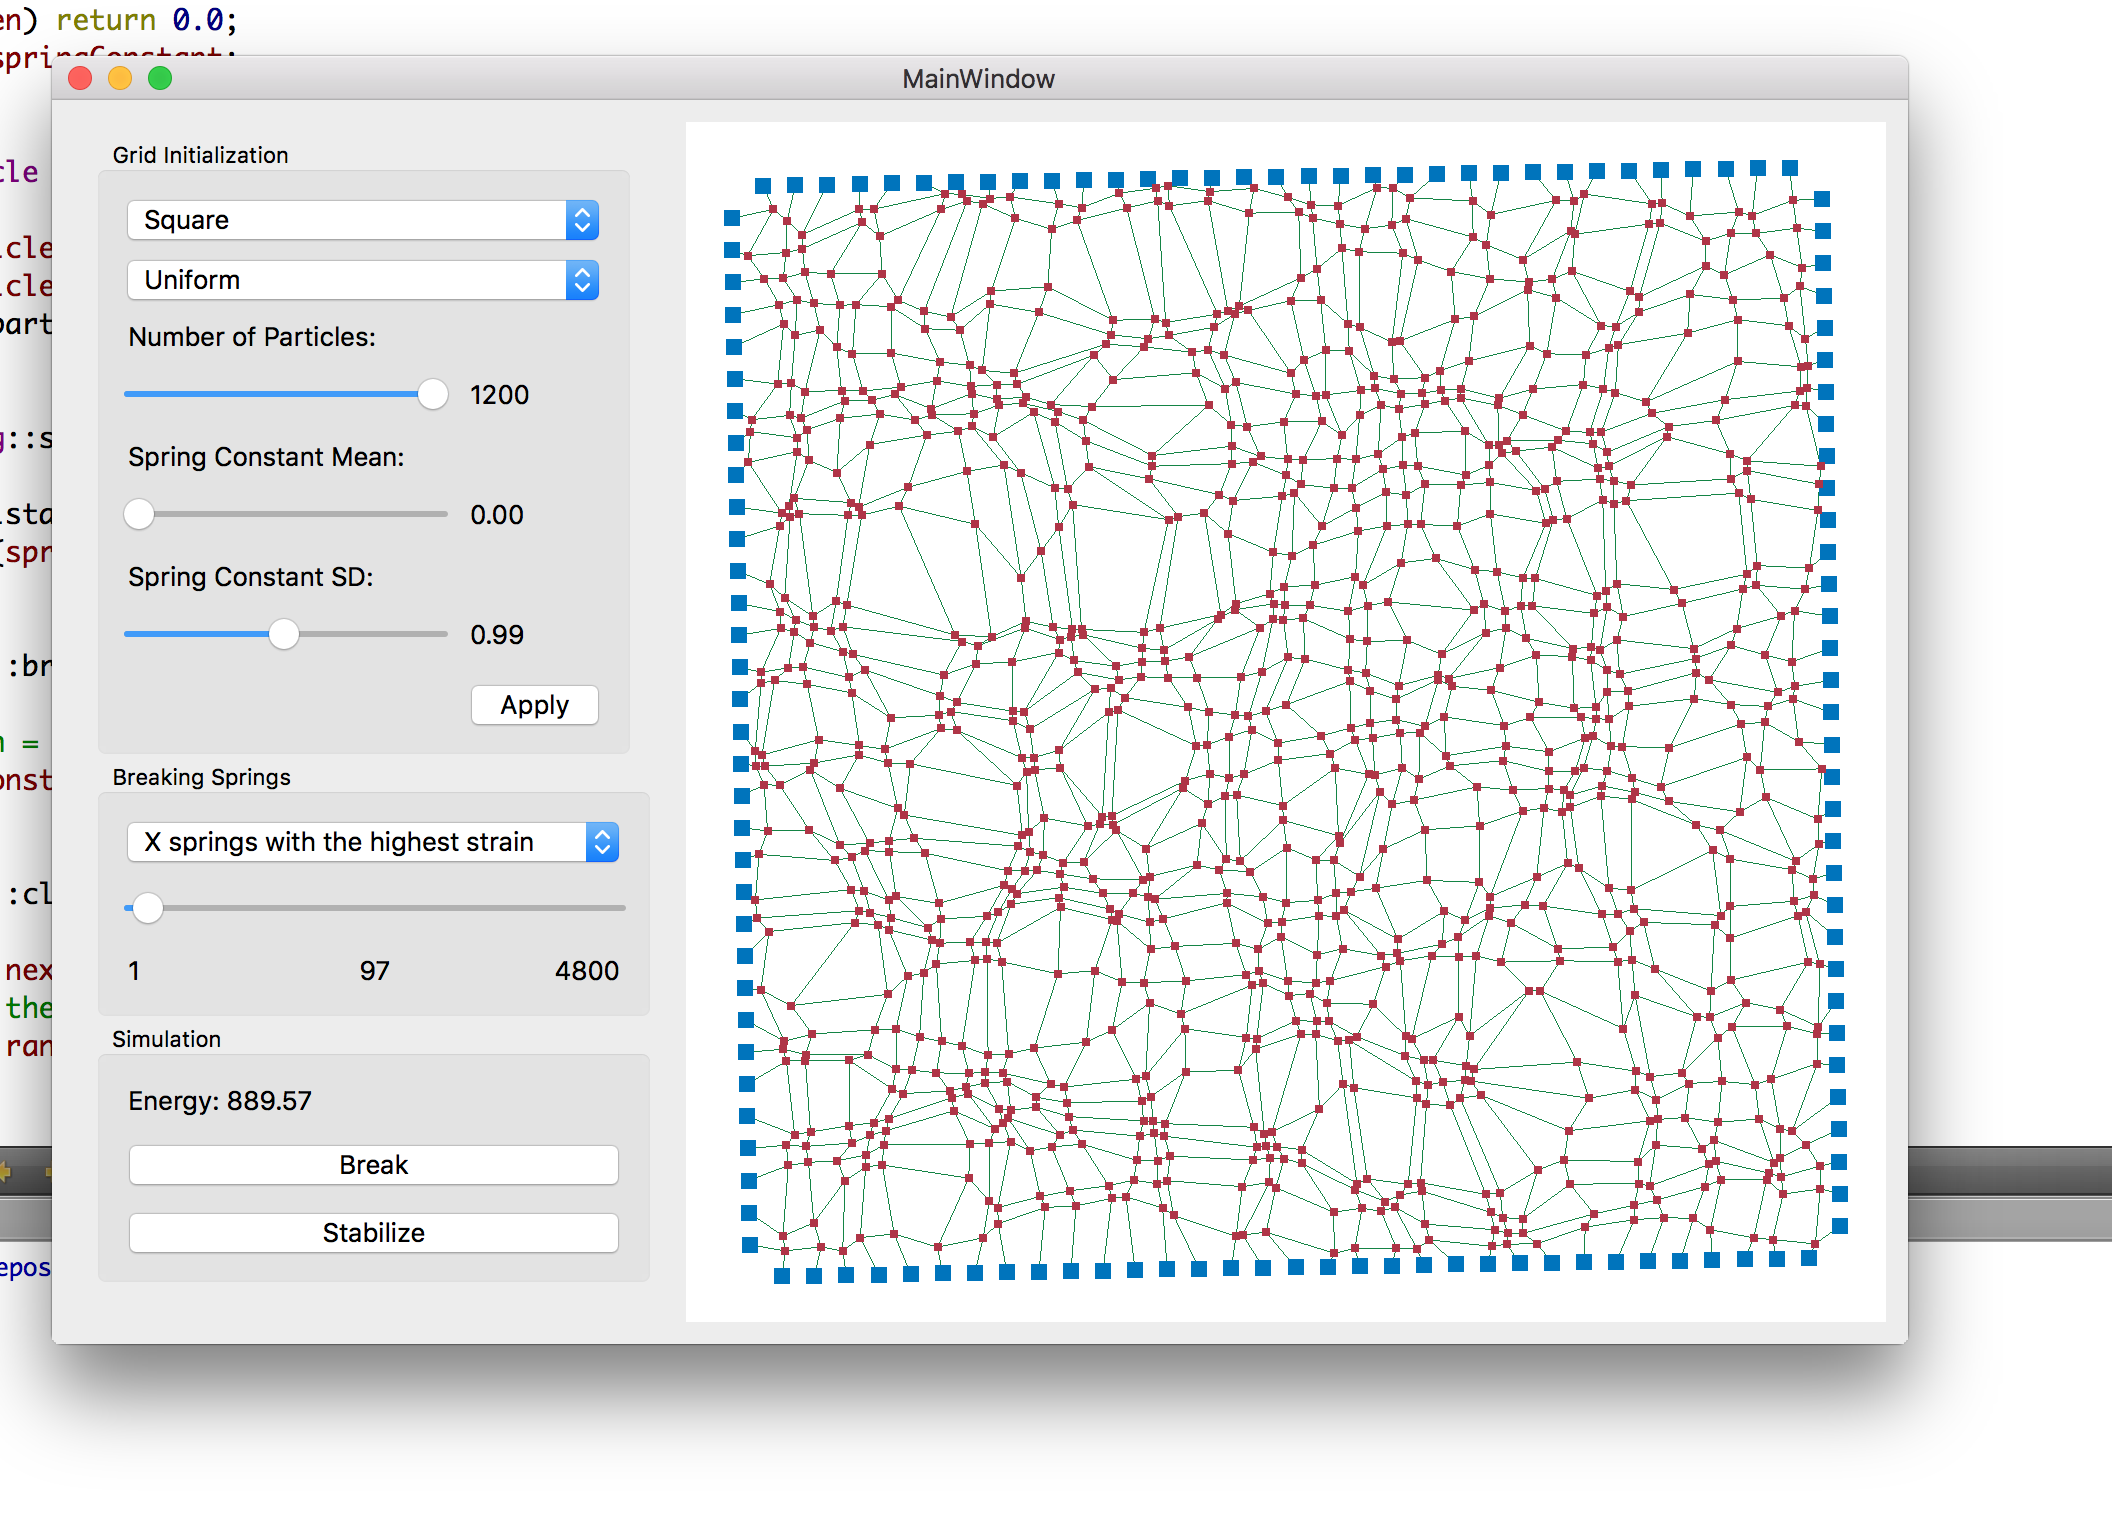
\includegraphics[
		width=\textwidth, 
		height=\textwidth, 
		keepaspectratio=true]
	{./img/results/1200_0_1_stretchHighest_97_step_5}
	%\caption{Step 4}
	%\label{fig:experiment:stretchHighestStrain:5}
\end{subfigure}

\begin{subfigure}{0.16\textwidth}
	\centering
	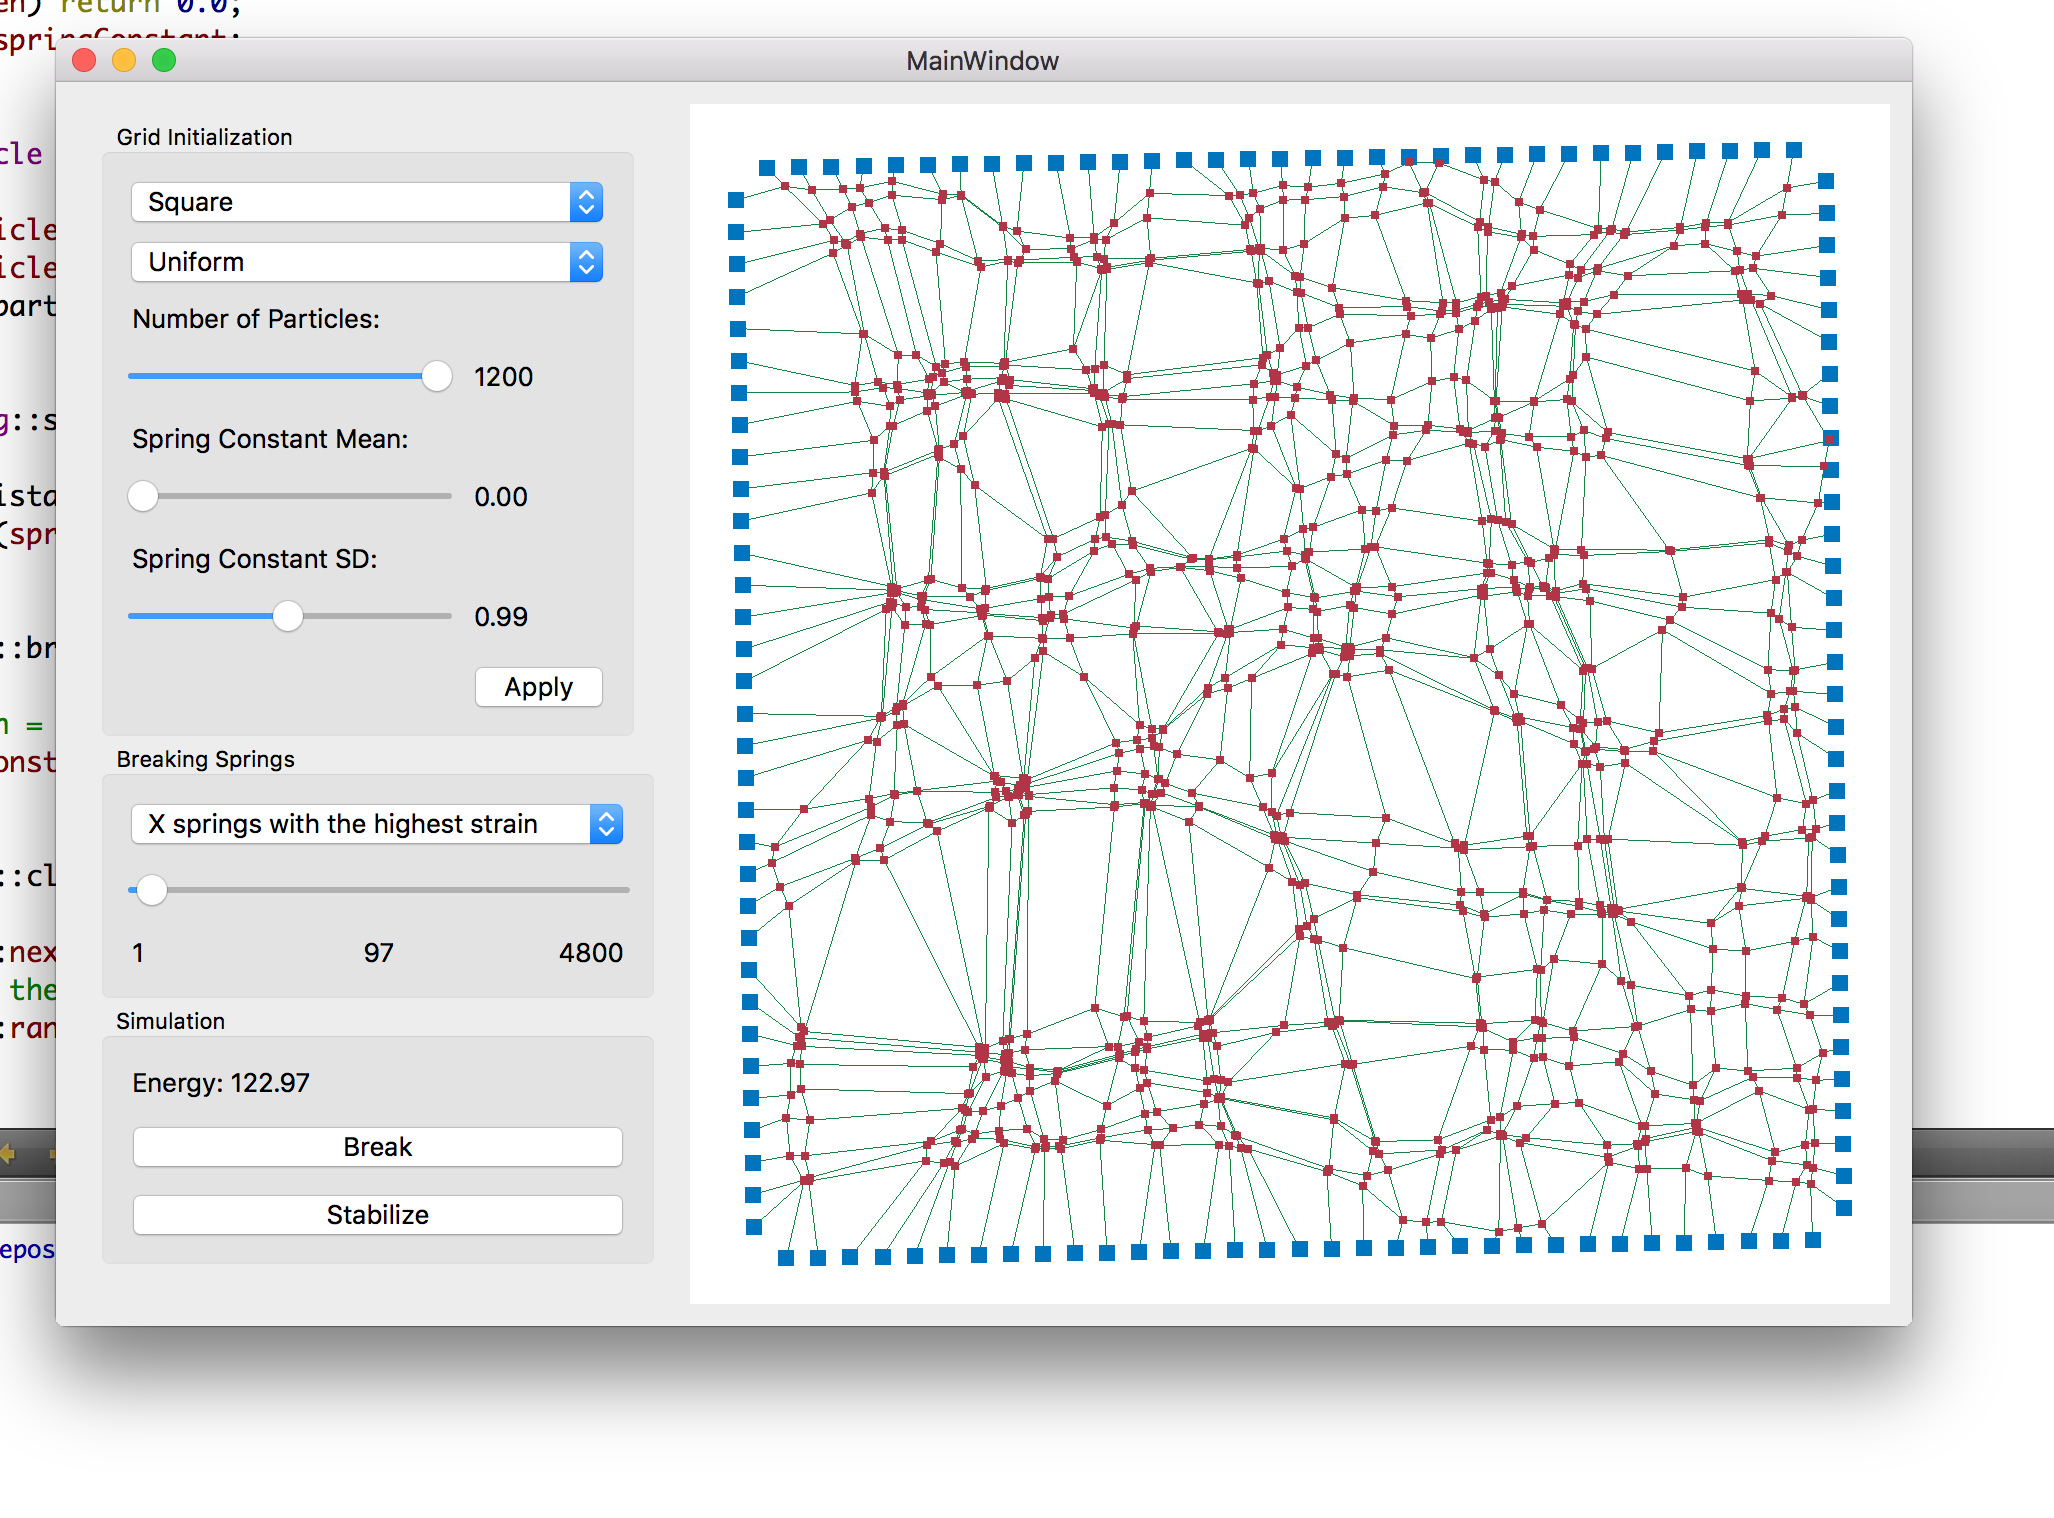
\includegraphics[
		width=\textwidth, 
		height=\textwidth, 
		keepaspectratio=true]
	{./img/results/1200_0_1_stretchHighest_97_step_50}
	%\caption{Step 50}
	%\label{fig:expe riment:stretchHighestStrain:50}
\end{subfigure}	
\begin{subfigure}{0.16\textwidth}
	\centering
	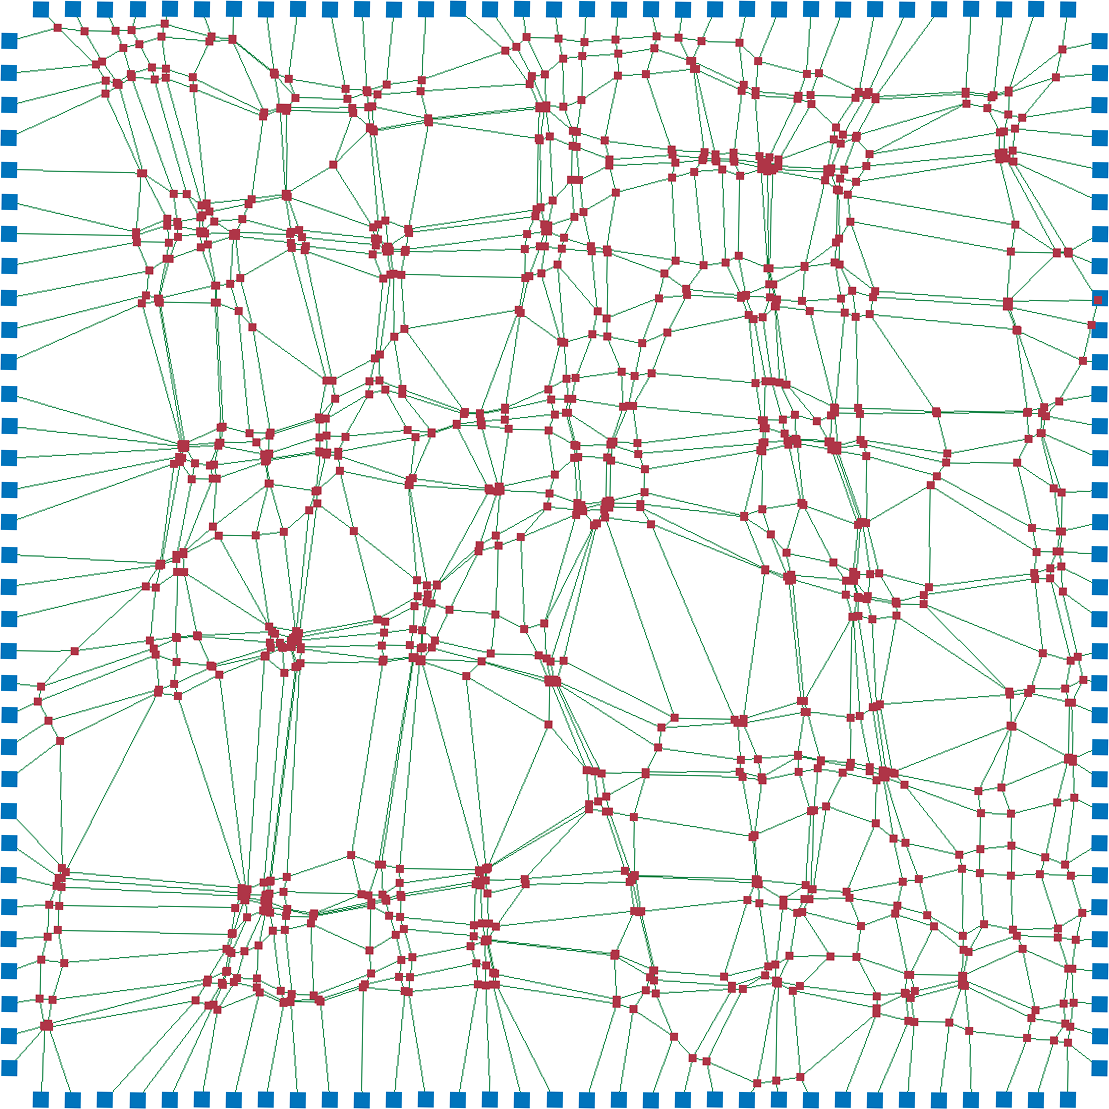
\includegraphics[
		width=\textwidth, 
		height=\textwidth, 
		keepaspectratio=true]
	{./img/results/1200_0_1_stretchHighest_97_step_51}
	%\caption{Step 51}
	%\label{fig:experiment:stretchHighestStrain:51}
\end{subfigure}		
\begin{subfigure}{0.16\textwidth}
	\centering
	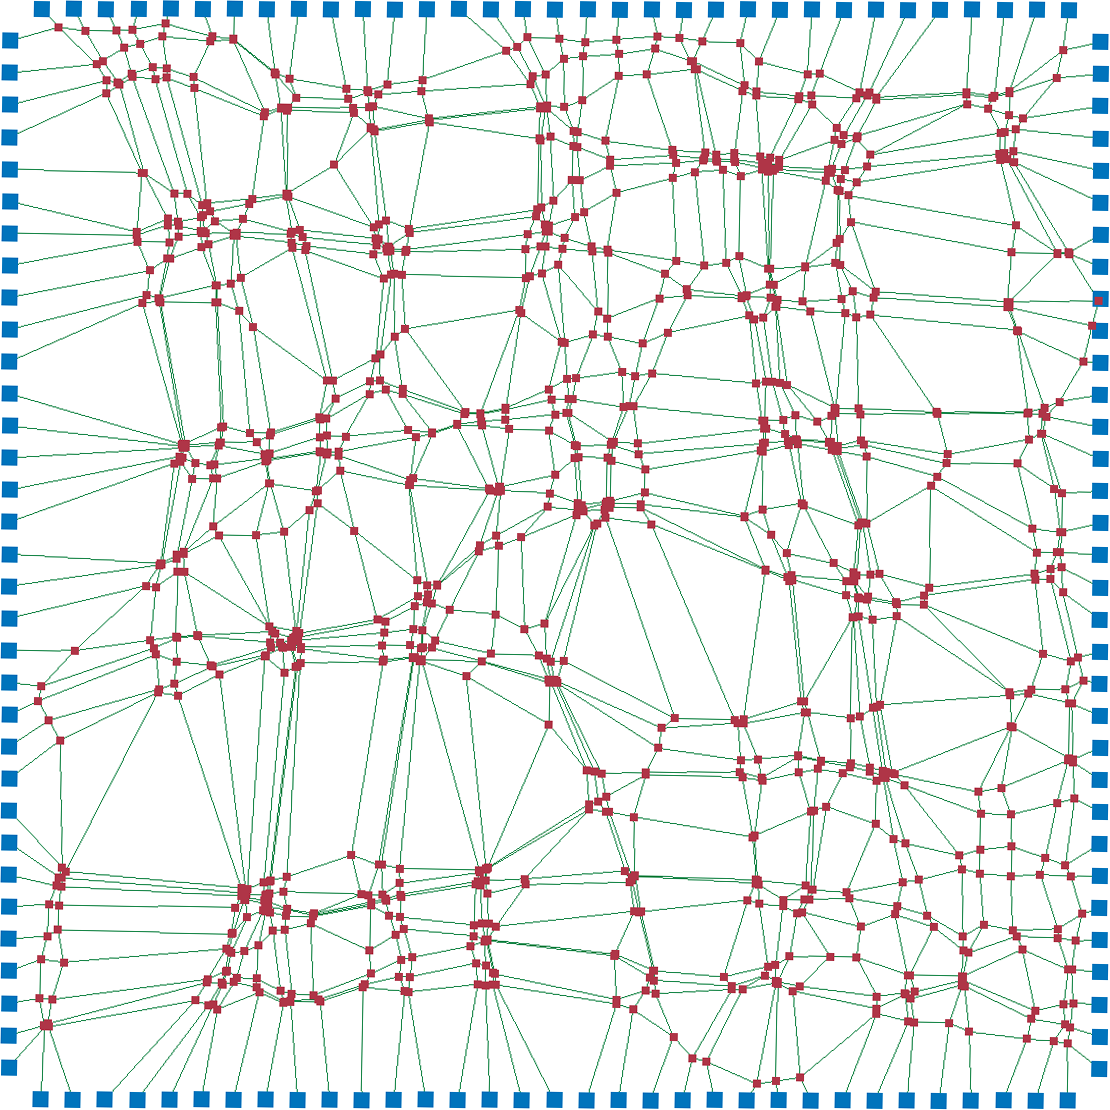
\includegraphics[
		width=\textwidth, 
		height=\textwidth, 
		keepaspectratio=true]
	{./img/results/1200_0_1_stretchHighest_97_step_52}
	%\caption{Step 52}
	%\label{fig:experiment:stretchHighestStrain:52}
\end{subfigure}			
\begin{subfigure}{0.16\textwidth}
	\centering
	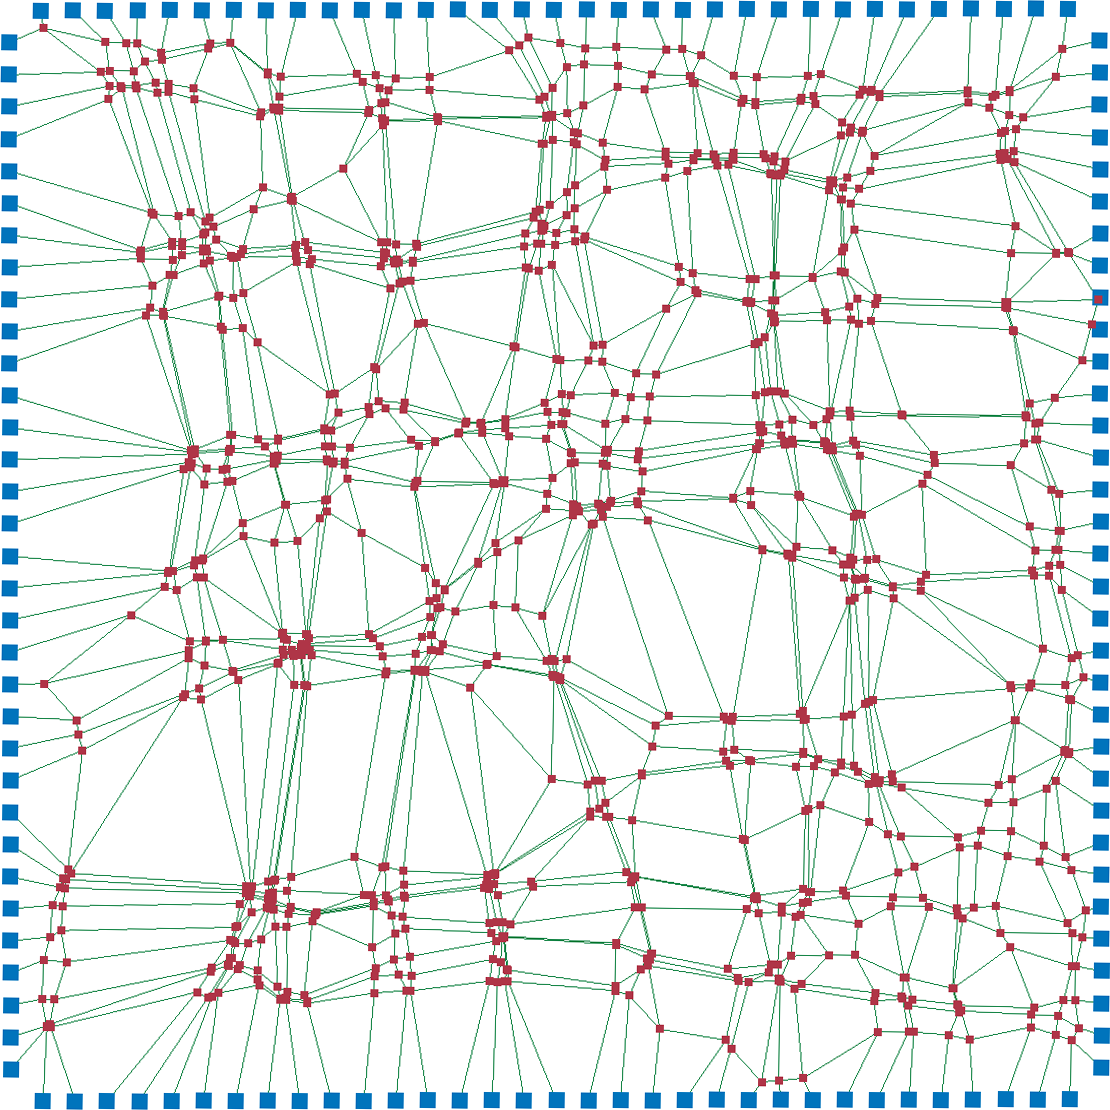
\includegraphics[
		width=\textwidth, 
		height=\textwidth, 
		keepaspectratio=true]
	{./img/results/1200_0_1_stretchHighest_97_step_53}
	%\caption{Step 53}
	%\label{fig:experiment:stretchHighestStrain:53}
\end{subfigure}				
\begin{subfigure}{0.16\textwidth}
	\centering
	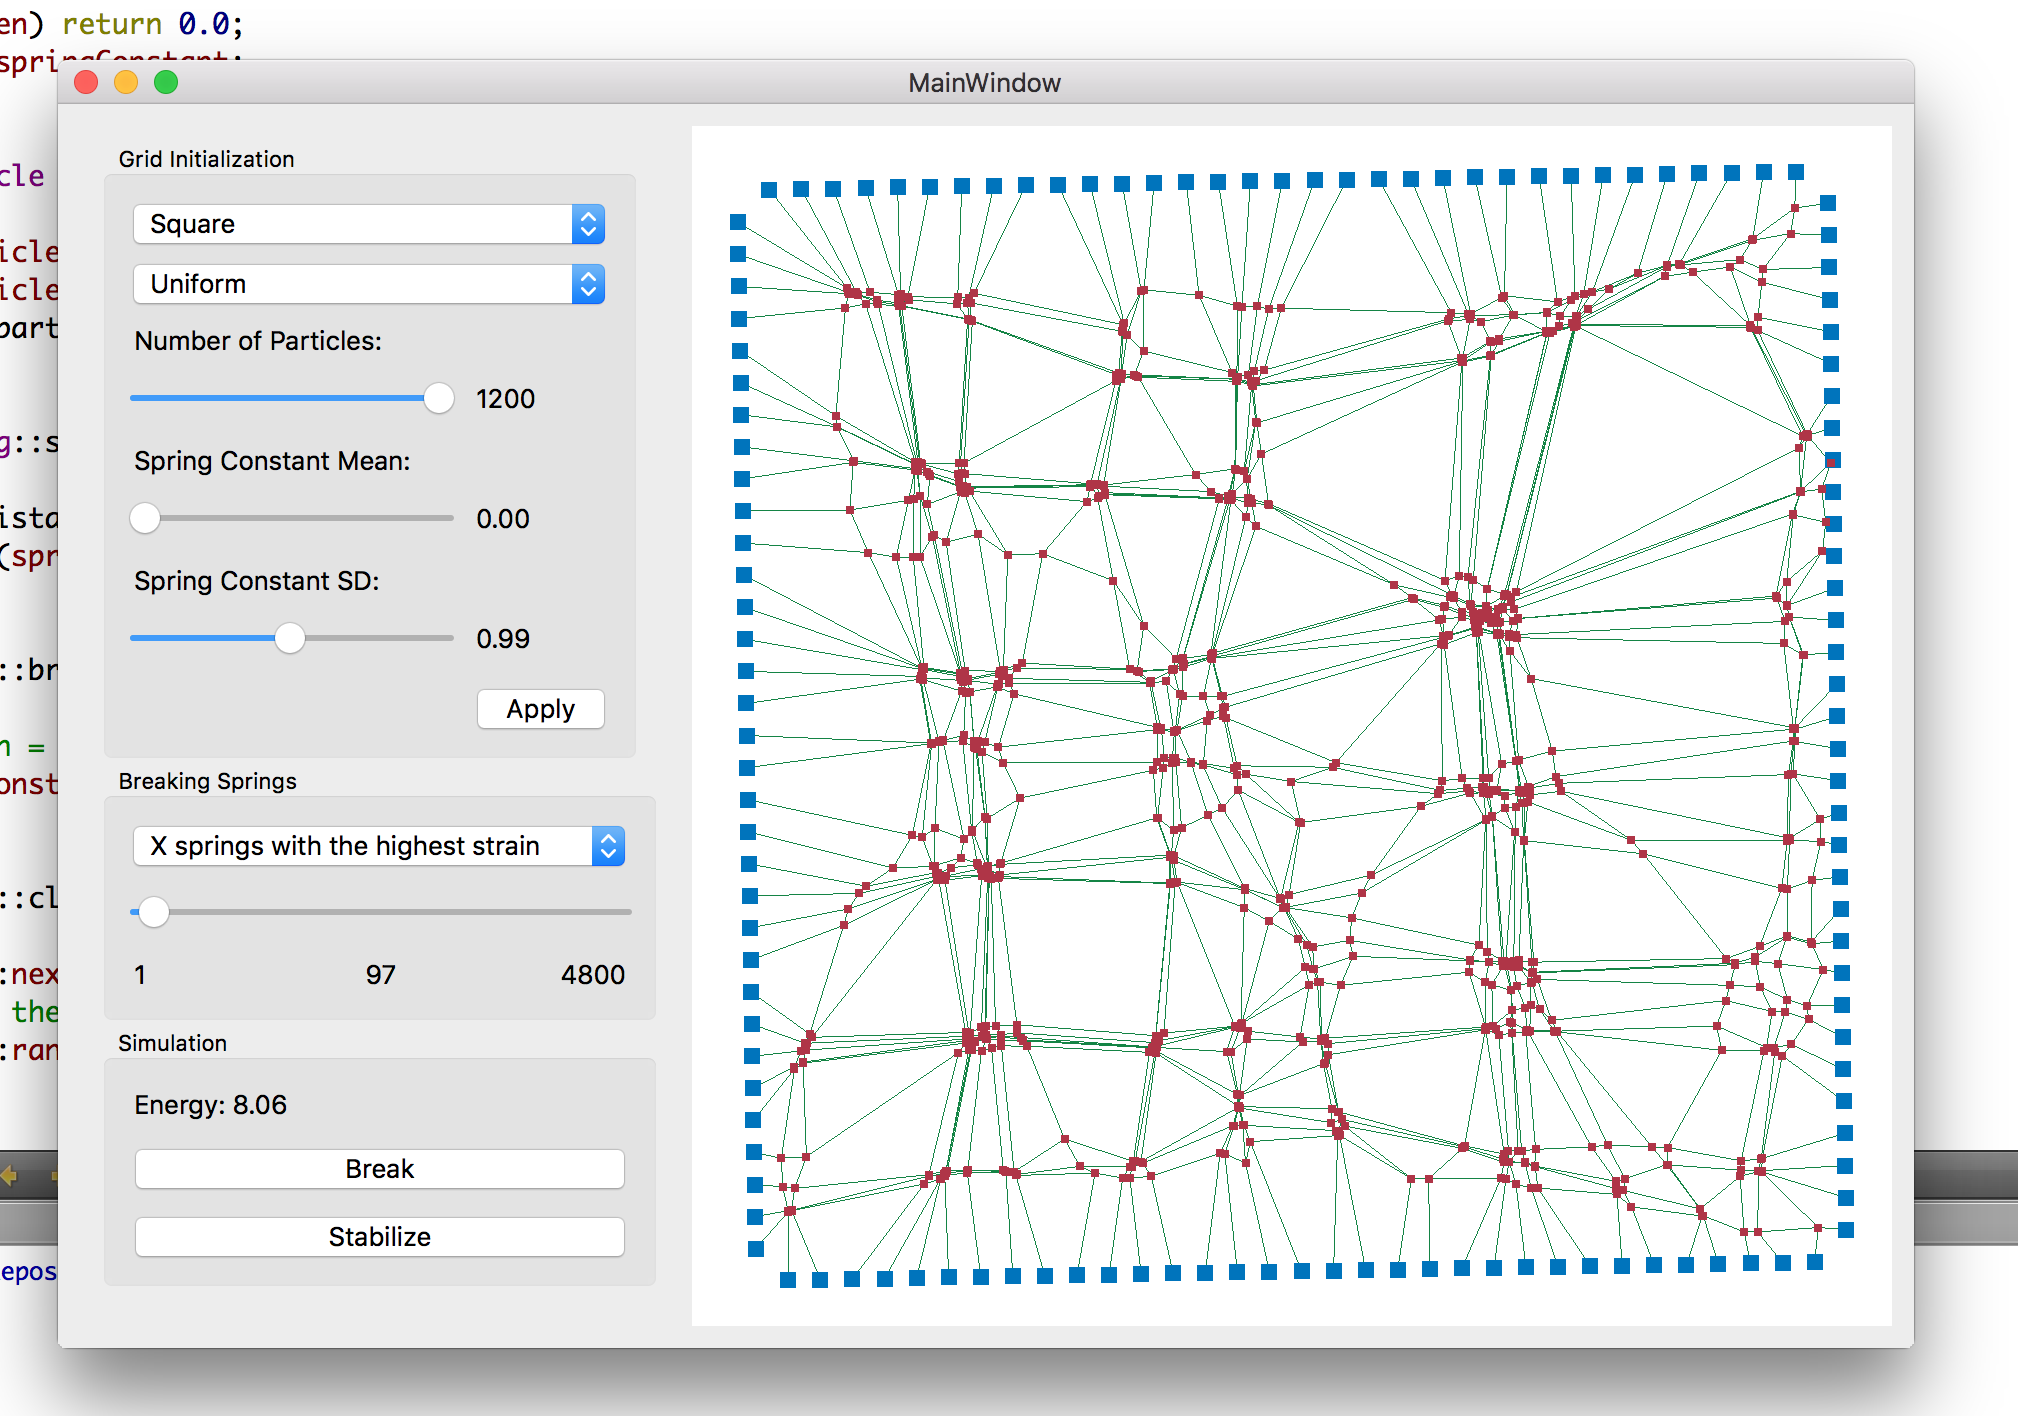
\includegraphics[
		width=\textwidth, 
		height=\textwidth, 
		keepaspectratio=true]
	{./img/results/1200_0_1_stretchHighest_97_step_80}
	%\caption{Step 80}
	%\label{fig:experiment:stretchHighestStrain:80}
\end{subfigure}
\begin{subfigure}{0.16\textwidth}
	\centering
	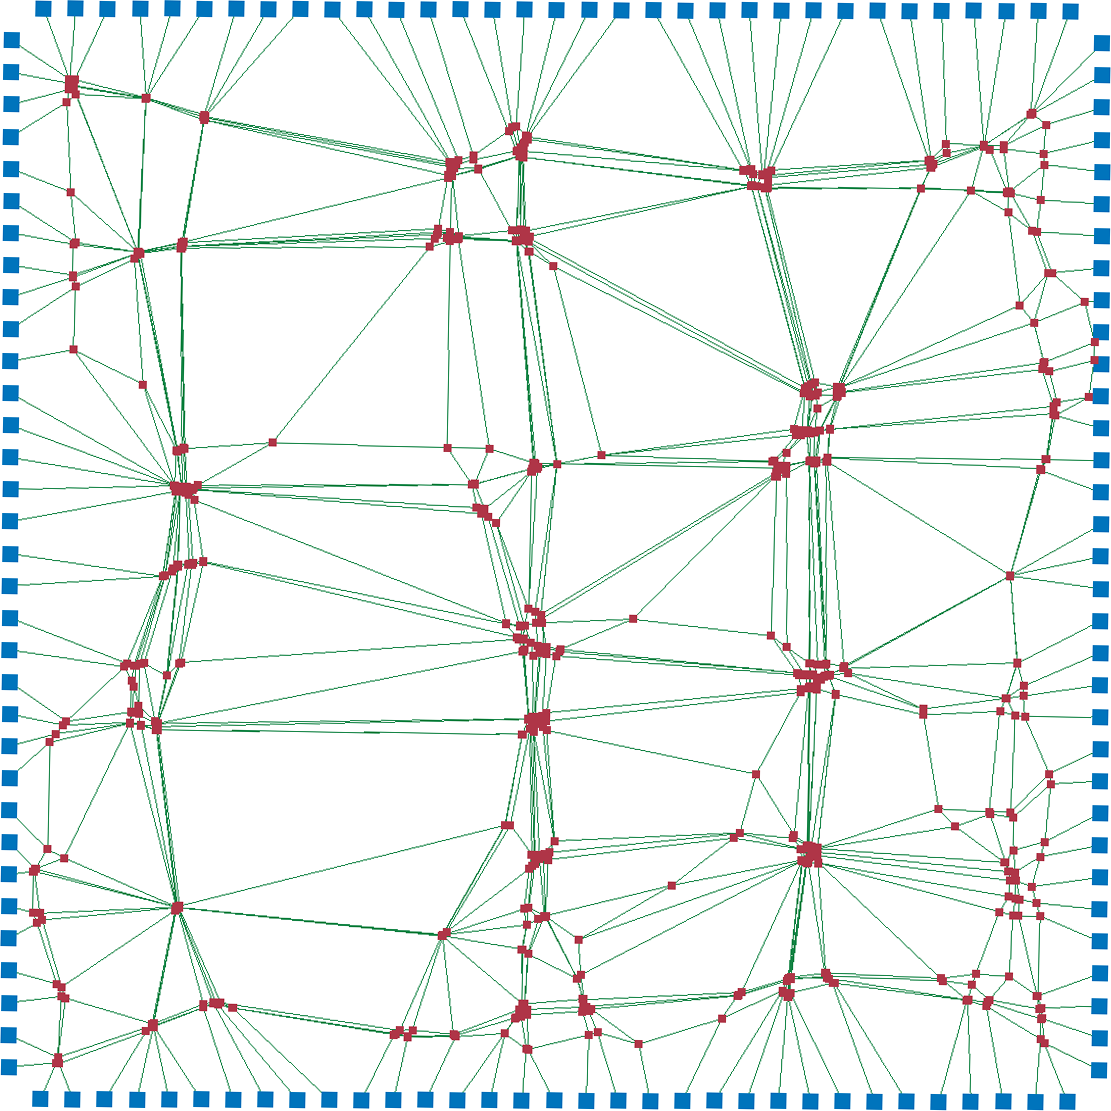
\includegraphics[
		width=\textwidth, 
		height=\textwidth, 
		keepaspectratio=true]
	{./img/results/1200_0_1_stretchHighest_97_step_100}
	%\caption{Step 100}
	%\label{fig:experiment:stretchHighestStrain:100}
\end{subfigure}